\begin{figure}[p]
\centering
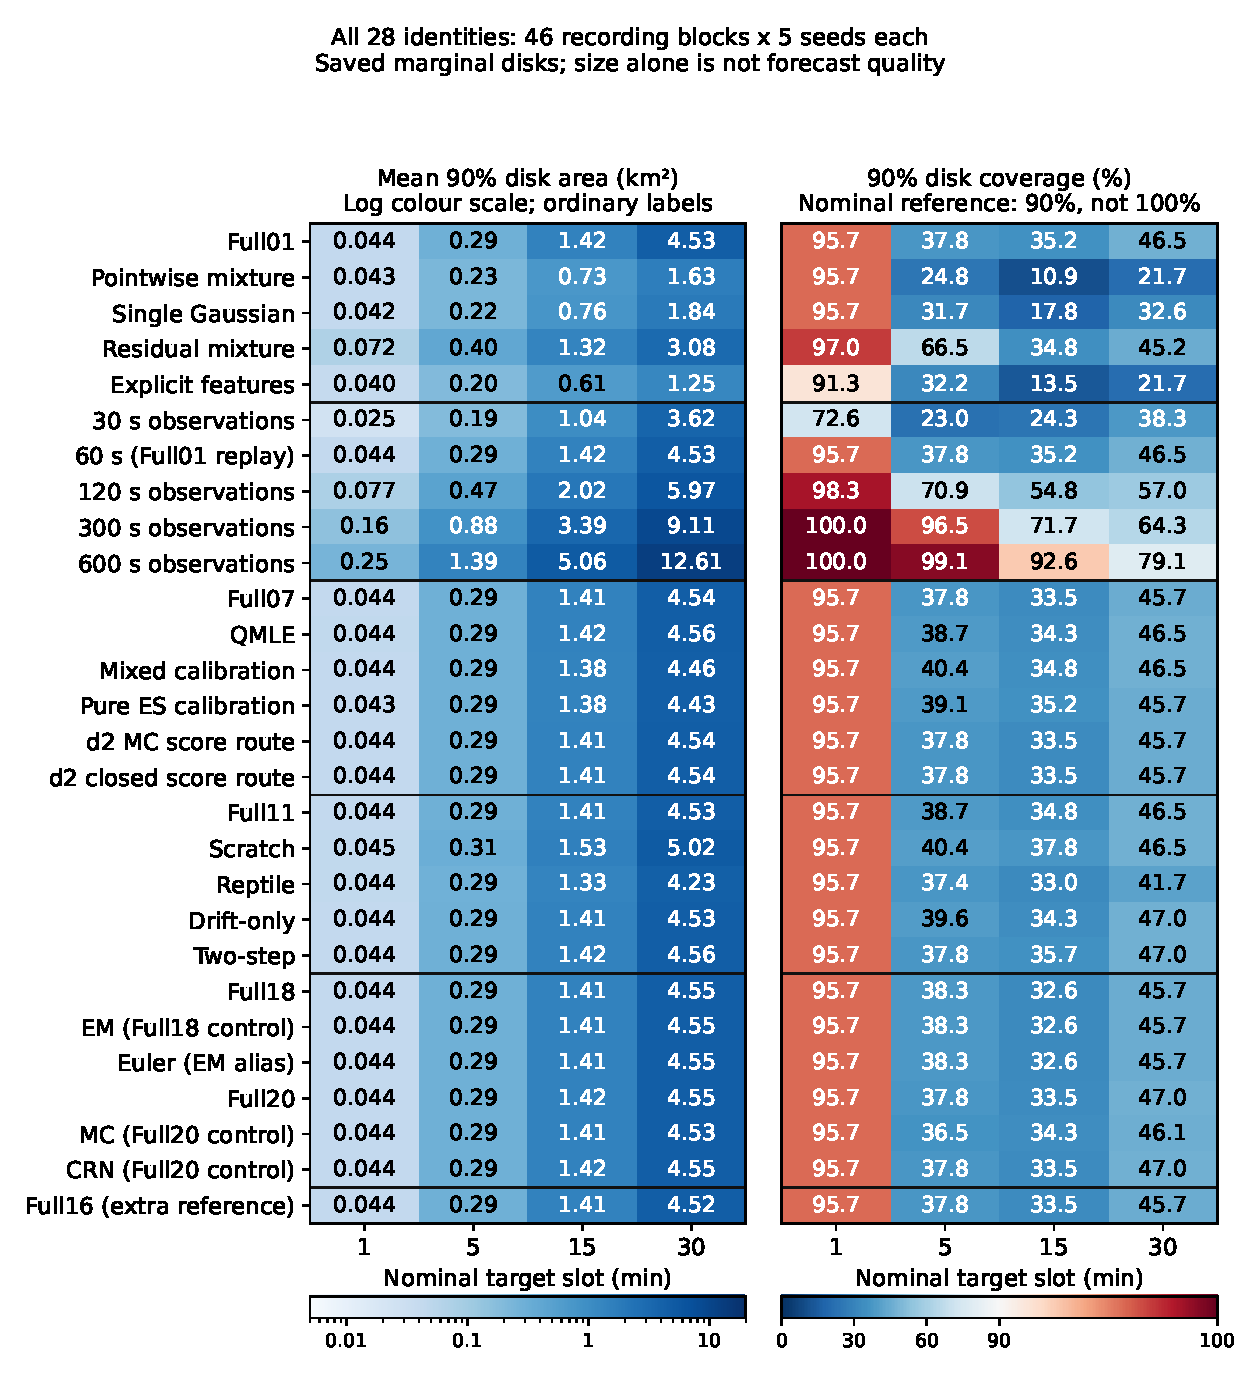
\includegraphics[height=.76\textheight,width=\linewidth,keepaspectratio]{../figures/revision46-corrections-v1/method-region-overview.pdf}
\caption{Complete 28-configuration region-size and coverage display at four original target slots. Left: mean nominal 90\% disk area (km$^2$); colour uses a logarithmic scale to show both short- and long-horizon areas, while cell labels give ordinary areas. Right: empirical target containment (\%), whose nominal reference is 90\%, not 100\%. Neither area nor coverage is a stand-alone quality ranking. Row order follows the declared method families, not observed performance; aliases and Full controls remain distinct. Each cell averages five seeds within each of 46 blocks and then equally over blocks. Descriptive means without new tests, prediction or recalibration; radii and exact values appear in Table~\ref{tab:all-method-regions} and the saved aggregate.}
\label{fig:all-method-regions}
\end{figure}
